\section{Definizione del problema da risolvere}

Già negli anni '80 si iniziò a definire il concetto di \textit{agricoltura di precisione}: un insieme di strategie e strumenti in grado di migliorare la produttività del suolo grazie all'impiego di sistemi satellitari e geo-referenziati. \`E stato quindi l'inizio del binomio \textit{tecnologia-agricoltura}, rafforzato con il termine \textit{agricoltura digitale}, fino ad arrivare all'\textit{agricoltura 4.0}\footnote{\url{https://www.bioaksxter.com/it/nuove-tecnologie-inizia-l-era-dell-agricoltura-4-0?module=blog&operazione=nuove-tecnologie-inizia-lera-dellagricoltura-4-0}}.

Questa innovazione tecnologica, perlomeno inizialmente, ha interessato specialmente le \textit{grandi coltivazioni}, come quelle di aziende agricole specializzate o grandi coltivazioni, anche se negli ultimi anni si stanno affacciando sul mercato alcuni tentativi di portare queste innovazioni all'interno di ambienti domestici.

Moltissimi privati, nella propria abitazione, dispongono di piante o vorrebbero averne, specialmente in questi tempi in cui la pandemia e le restrizioni dovute ad essa hanno fatto si che la coltivazione di piccoli spazi verdi abbia assunto un ruolo fondamentale per le persone. Infatti, secondo il sito \texttt{businessintelligencegroup}\footnote{\url{https://www.businessintelligencegroup.it/quanto-vale-il-mercato-del-giardinaggio-in-italia/}}, "\textit{oltre il 60\% delle persone che possiede un’area green (giardino, ma anche terrazzo, veranda o orto) la apprezza e la sfrutta con molta più frequenza rispetto al passato}".

Tuttavia, le piante sono organismi delicati che richiedono cure costanti e attenzioni, ma anche di competenze. In quest'ottica, la diffusione di dispositivi intelligenti a supporto della \textit{coltivazione domestica} di piccole piante è fondamentale per supportare gli appassionati, ma anche le persone che vorrebbero approcciarsi al mondo \textit{green}.

\begin{figure}[h!]
	\centering
	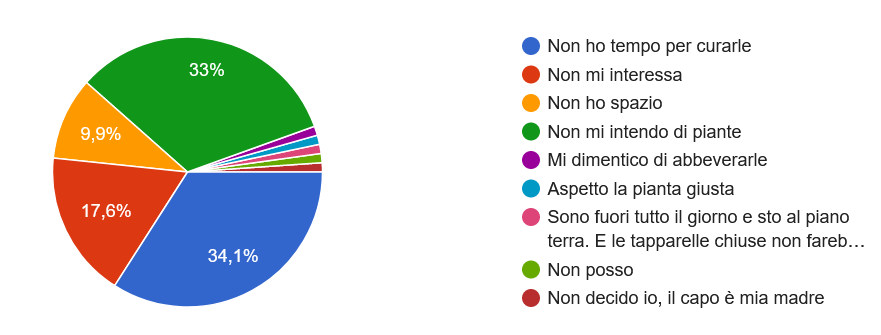
\includegraphics[width=\columnwidth]{images/torta_perche_no_piante.png}
	\caption{Dati raccolti sulle motivazioni di chi non dispone di piante nella propria abitazione}
	\label{fig:whynot}
\end{figure}

Una piccola indagine svolta da noi mostra che, su un campione di 269 privati, quasi il 35\% non possiede una pianta in casa in quanto non ha il tempo e/o le competenze necessarie (fig.\ref{fig:whynot}).
Risulta quindi chiaro che molte persone \textit{vorrebbero} avere una o più piante in casa, ma non riescono a causa dei motivi sopra descritti.

In quest'ottica, nasce un forte bisogno di un prodotto o servizio che possa aiutare queste persone a colmare le carenze di tempo e competenze, in modo da permettere anche a loro di godere dei benefici che scaturiscono dalla coltivazione di una pianta. Questo però, senza fargli \textit{perdere il contatto} con il senso stesso dell'arte della coltivazione di una pianta e che quindi non si sostituisca completamente all'uomo.

Se infatti tutti coloro che non sono immersi nel mondo dell'agricoltura lamentano l'assenza di tempo e competenze, anche gli appassionati potrebbero trarre notevole beneficio da meccanismi di supporto alla crescita delle proprie piante, in quanto potrebbero rappresentare un'opportunità per estendere il proprio\textit{ bagaglio di conoscenze}.

Nasce a questo proposito il bisogno di un prodotto che sia utilizzabile anche da chi dispone di proprie attrezzature, come ad esempio vasi dei quali non vuole sbarazzarsi.
Riteniamo quindi l'adattabilità un aspetto e un problema chiave nello sviluppo di un dispositivo di questo tipo.

Per concludere, possiamo sintetizzare i principali problemi che abbiamo identificato ed esposto, in questi tre punti chiave:
\begin{enumerate}
	\item \textbf{Pochi prodotti \textit{entry level}} a supporto della coltivazione di piante di \textit{piccola/media taglia};
	
	\item \textbf{Tempo e competenze necessarie}, dalle nostre indagini è emerso che spesso le persone non hanno tempo di occuparsi delle piante oppure non hanno le competenze necessarie per prendersene cura;
	
	\item \textbf{Scarsa adattabilità}, i prodotti smart esistenti non sono utilizzabili su attrezzature (vasi, fioriere, serre) già in possesso del cliente.
\end{enumerate}
